\documentclass{article}
\usepackage{tikz}
\begin{document}

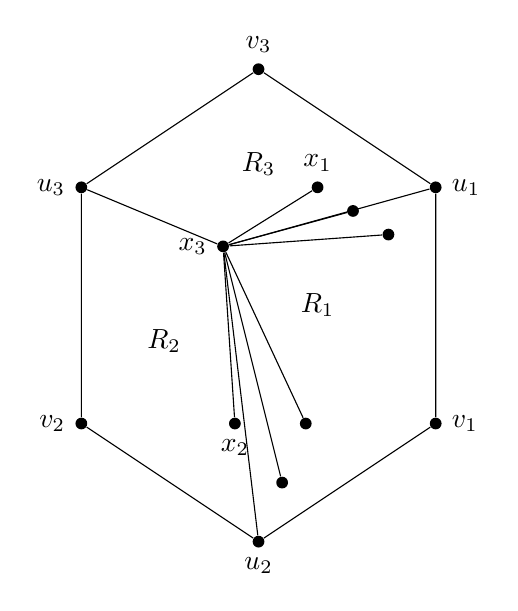
\begin{tikzpicture}[scale=1.5]
    % Define vertices
    \node[circle, fill=black, inner sep=1.5pt, label=right:$u_1$] (u1) at (3,2) {};
    \node[circle, fill=black, inner sep=1.5pt, label=right:$v_1$] (v1) at (3,0) {};
    \node[circle, fill=black, inner sep=1.5pt, label=below:$u_2$] (u2) at (1.5,-1) {};
    \node[circle, fill=black, inner sep=1.5pt, label=left:$v_2$] (v2) at (0,0) {};
    \node[circle, fill=black, inner sep=1.5pt, label=left:$u_3$] (u3) at (0,2) {};
    \node[circle, fill=black, inner sep=1.5pt, label=above:$v_3$] (v3) at (1.5,3) {};
    
    % Define interior vertices
    \node[circle, fill=black, inner sep=1.5pt, label=above:$x_1$] (x1) at (2,2) {};
    \node[circle, fill=black, inner sep=1.5pt, label=below:$x_2$] (x2) at (1.3,0) {};
    \node[circle, fill=black, inner sep=1.5pt, label=left:$x_3$] (x3) at (1.2,1.5) {};
    
    % Additional vertices near u1
    \node[circle, fill=black, inner sep=1.5pt] (p1) at (2.3,1.8) {};
    \node[circle, fill=black, inner sep=1.5pt] (p2) at (2.6,1.6) {};
    
    % Additional vertices near u2
    \node[circle, fill=black, inner sep=1.5pt] (q1) at (1.7,-0.5) {};
    \node[circle, fill=black, inner sep=1.5pt] (q2) at (1.9,0) {};
    
    % Draw the hexagon edges
    \draw (u1) -- (v1) -- (u2) -- (v2) -- (u3) -- (v3) -- (u1);
    
    % Draw connections from x3
    \draw (x3) -- (u1);
    \draw (x3) -- (p1);
    \draw (x3) -- (p2);
    \draw (x3) -- (x1);
    \draw (x3) -- (u3);
    \draw (x3) -- (u2);
    \draw (x3) -- (q1);
    \draw (x3) -- (q2);
    \draw (x3) -- (x2);
    
    % Label the regions
    \node at (2,1) {$R_1$};
    \node at (0.7,0.7) {$R_2$};
    \node at (1.5,2.2) {$R_3$};
    
\end{tikzpicture}

\end{document}